The fourth observing run started on the 24th May 2023 with only the two LIGO detectors taking data, Virgo needing some more time to reach the expected sensitivity.
This means that there were only single and double detector time.
Figure \ref{fig:dc_O4} shows the duty cycle of the detector network from the 24th May 2023 (GPS=1368933107) to the 9th July 2023 (GPS=1372947450) ($\sim 46.5$ days).
We give here an overview of the results of the single detector search for this period of time.

\begin{figure}[hb]
  \centering
  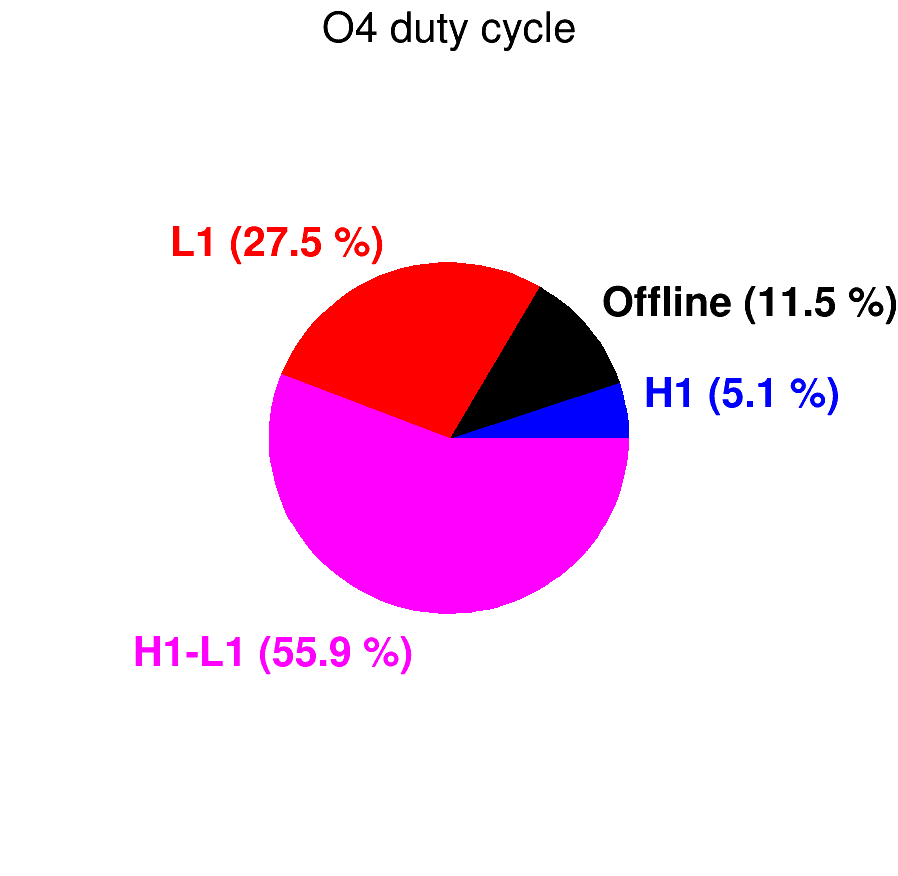
\includegraphics[width=0.5\linewidth]{sectionO4/cDutyCycle.png}
  \caption{Detector network duty cycle for the first 46.5 days of O4.}
  \label{fig:dc_O4}
\end{figure}


%%%%%%%%%%
\subsection{Effectiveness of the selection criteria}
We first want to check whether the single detector selection criteria defined previously worked as intended.
In this chapter, we exclude all single detector triggers that are associated to a significant public alert.
Figures \ref{fig:all_singles_O4} shows all single detector triggers for the same period of time as the duty cycle figure.
Note that we do not distinguish here between background triggers and the few triggers that are likely to be of astrophysical origin.

Figure \ref{fig:tempdur_O4} shows the rwSNR vs template duration distribution (starting from 24 Hz, or 20 Hz for the high mass one band templates) of those single detector triggers.
We can see that there are still some short templates which produce many triggers with sometimes high rwSNR.

For the single detector analysis done on O3 data, we defined the EM bright population to restrain the parameter space and reduce the background.
The population was defined based on the chirp mass and mass1 of the systems in such a way that it would be similar to a selection on $\text{hasRemnant}>0.1\%$.
This was because we did not compute hasRemnant during O3.
For O4, the hasRemnant quantity is computed by MBTA.
The EM bright population is therefore taken as $\text{hasRemnant}>0.1\%$.
This definition includes 87\% of the templates of the O4 bank.

Figure \ref{fig:tempdur_embright_O4} shows the rwSNR vs template duration for EM bright single detector triggers.
We see that the noisy templates seen in figure \ref{fig:tempdur_O4} are not part of the EM bright population.

Looking at figure \ref{fig:embright_O4}, which shows the rwSNR distribution of EM bright single detector triggers before and after the selection criteria defined in chapter \ref{section:selection}.
We see that the selection criteria reduce the overall number of triggers, especially in L1 where many high rwSNR trigger are rejected.
With the selection criteria applied, the distribution of EM brigth triggers follows an exponential shape with a few outliers in L1.
Most of them have a very asymmetric template in terms of masses.
Adding an extra selection on the mass ratio $m_1/m_2<30$ allows to remove these triggers as shown in figure \ref{fig:embright_O4}.
Furthermore, some changes to the gating that occured after the detection of these triggers allows to remove two of them when analyzing the data offline with the latest MBTA configuration.

%%%%%%%%%%% EM BRIGHT SELECTION
\begin{figure}
  \centering
  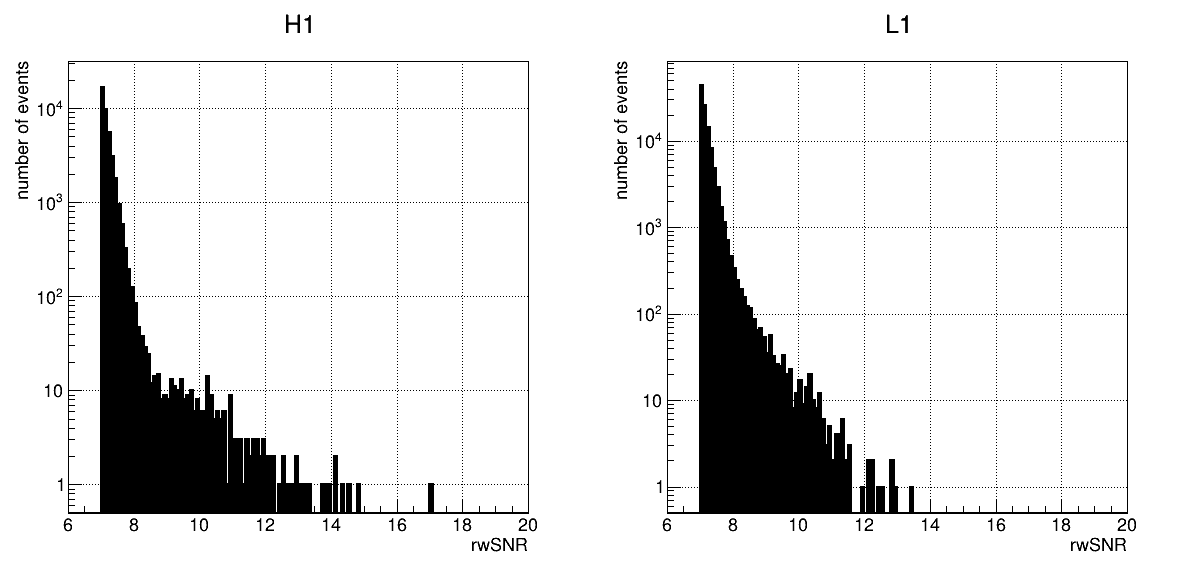
\includegraphics[width=\linewidth]{sectionO4/cRwSnrO4.png}
  \caption{rwSNR distribution of all single detector triggers for the first 46.5 days of O4.
  Effective times in H1 and L1 are 28.4 days and 38.7 days respectively. Triggers associated to significant public alerts were removed.}
  \label{fig:all_singles_O4}
\end{figure}
%
\begin{figure}
  \centering
  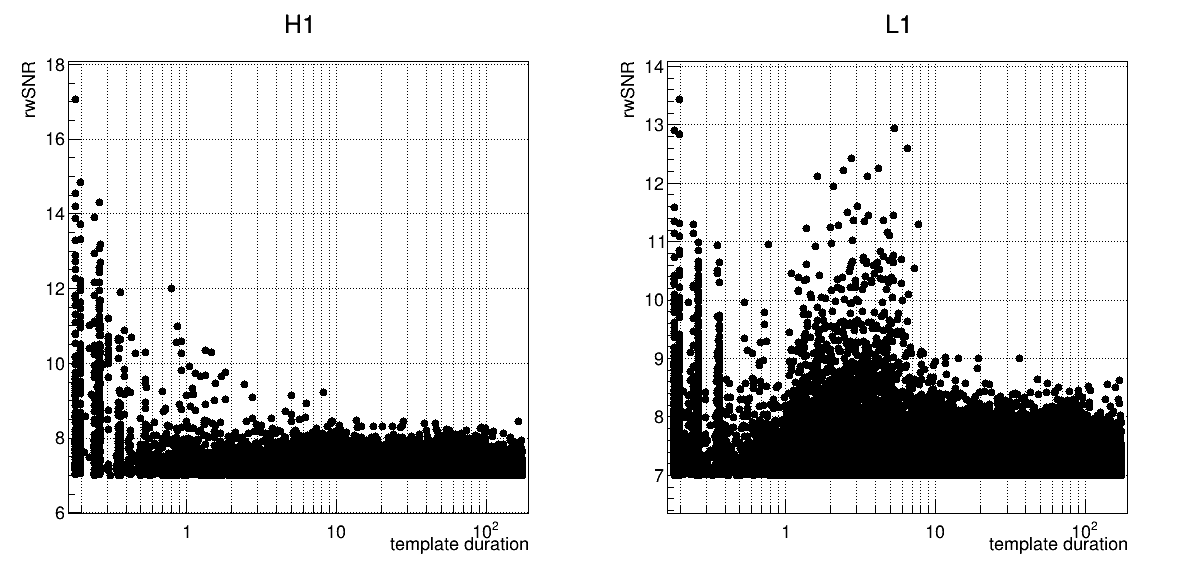
\includegraphics[width=\linewidth]{sectionO4/cSnrTempDur_all.png}
  \caption{rwSNR vs template duration distribution of all single detector triggers for the first 46.5 days of O4. Triggers associated to significant public alerts were removed.}
  \label{fig:tempdur_O4}
\end{figure}
%
\begin{figure}
  \centering
  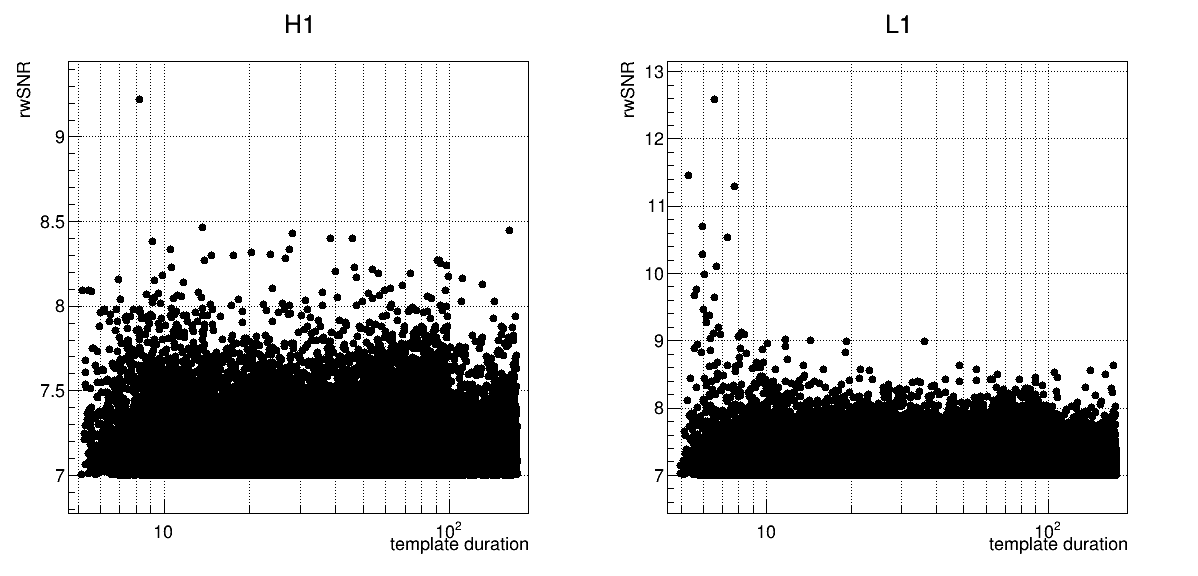
\includegraphics[width=\linewidth]{sectionO4/cSnrTempDur_bright.png}
  \caption{rwSNR vs template duration distribution of EM bright single detector triggers for the first 46.5 days of O4. Triggers associated to significant public alerts were removed.}
  \label{fig:tempdur_embright_O4}
\end{figure}
%
\begin{figure}
  \centering
  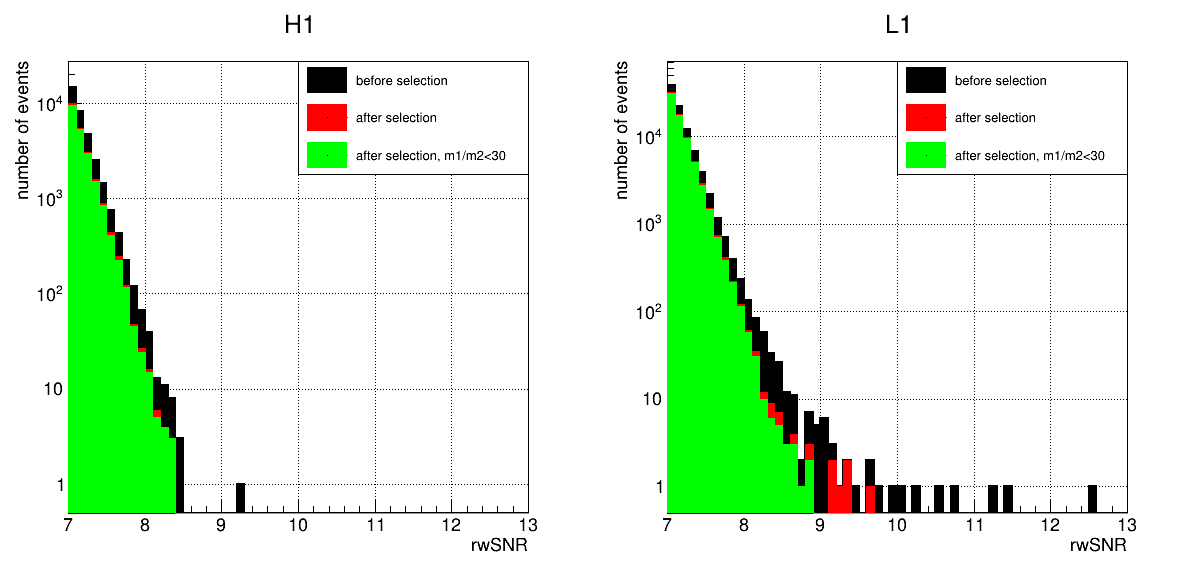
\includegraphics[width=\linewidth]{sectionO4/cRwSnr_bright.png}
  \caption{rwSNR distribution of EM bright single detector triggers for the first 46.5 days of O4 (28.4 effective days in H1 and 38.7 effective days in L1). Black is before applying the selection criteria defined in chapter \ref{section:selection}. Red is after applying the criteria. Adding an extra selection on the mass ratio $m_1/m_2<30$ yields the green distribution. Triggers associated to significant public alerts were removed.}
  \label{fig:embright_O4}
\end{figure}
%

%%%%%%%%%%%%%%%% ER AND GATING CUTS

Another thing to be checked is the criteria themselves.
They were defined by looking at O3 background, which is different from O4 background.
In addition the pipeline went through some changes between the runs, with in particular a new template bank and modification to the gating.
The criteria were defined to be conservative and avoid sending false alerts at the begining of the run.
They may be improved to be more performant and/or cause less duty cycle loss.
Although we do not have a lot of data yet we can still have a first look.

Figures \ref{fig:cutER_bright_O4} and \ref{fig:cutGating_bright_O4} show the rwSNR for EM bright single detector triggers with several cuts on the excess rate and gating respectively.
As it can be seen the effect of the selection on the gating is marginal on this period of time.
The selection on the excess rate on the other hand allowed to reject some triggers.
We see that the time window in which we look for excess rate has a limited impact.
The same can be said about EM dark single detector triggers, as shown by figures \ref{fig:cutER_dark_O4} and \ref{fig:cutGating_dark_O4}.
The remaining duty cycle after applying the selection criteria on the ER or the gating are given in table \ref{tab:dc_cut_O4}.
This gives hope that we may be less stringent on the selection criteria for O4.
But we have to keep in mind that we have less than two month of data here.
Furthemore, the gating parameters have been changed after several weeks of operation, to better catch the low frequency noise fluctuation.
This reduces a bit the high SNR triggers, and could also change the distributions shown in this section when running offline with the new gating.



\begin{table}
  \centering
  \begin{tabular}{c|c|c||c|c|c}
    Excess rate cut & H1 & L1 & Gating & H1 & L1 \\ \hline
    $\left[-3;+3\right]$s & 89.8\% & 96.6\% & $\left[-5;+5\right]$s & 99.2\% & 99.4\% \\
    $\left[-5;+5\right]$s & 88.0\% & 95.9\% & $\left[-10;+5\right]$s & 98.8\% & 99.1\% \\
    $\boldsymbol{\left[-7;+7\right]}$\textbf{s} & \textbf{86.3\%} & \textbf{95.3\%} & $\left[-15;+5\right]$s & 98.4\% & 98.8\% \\
    $\left[-10;+10\right]$s & 83.8\% & 94.4\% & $\boldsymbol{\left[-20;+5\right]}$\textbf{s} & \textbf{98.0\%} & \textbf{98.5\%} \\
  \end{tabular}
  \caption{Duty cycle left after applying a selection on the gating or the excess rate.
  For the analysis on O3 data we used $\left[-7;+7\right]$s for the selection on the excess rate and $\left[-20;+5\right]$s for the selection on the gating.}
  \label{tab:dc_cut_O4}
\end{table}

\begin{figure}
  \centering
  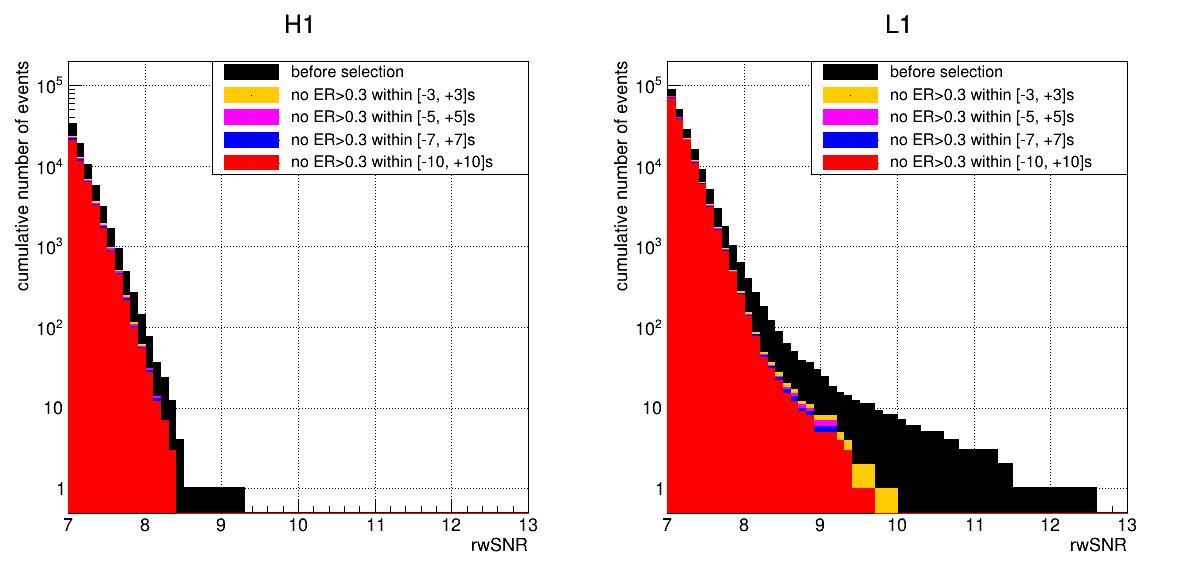
\includegraphics[width=\linewidth]{sectionO4/compareCutER_bright.png}
  \caption{Cumulative rwSNR distribution of EM bright single detector triggers for the first 46.5 days of O4 (28.4 effective days in H1 and 38.7 effective days in L1) for several cuts on the excess rate. No selection on the gating is applied here. Triggers associated to significant public alerts were removed.}
  \label{fig:cutER_bright_O4}
\end{figure}
%
\begin{figure}
  \centering
  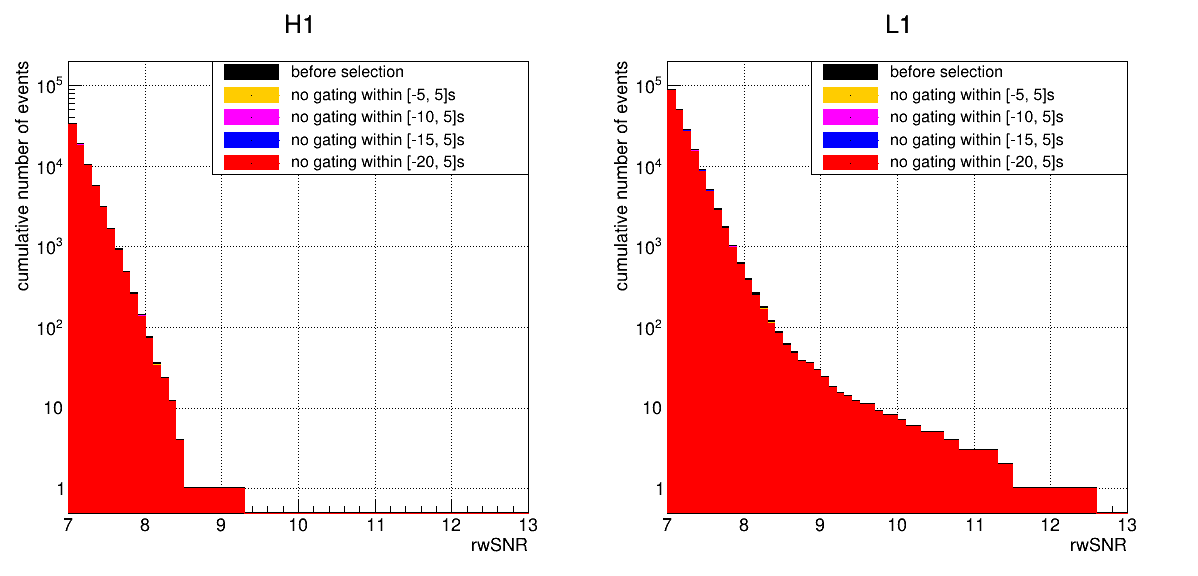
\includegraphics[width=\linewidth]{sectionO4/compareCutGating_bright.png}
  \caption{Cumulative rwSNR distribution of EM bright single detector triggers for the first 46.5 days of O4 (28.4 effective days in H1 and 38.7 effective days in L1) for several cuts on the gating. No selection on the ER is applied here. Triggers associated to significant public alerts were removed.}
  \label{fig:cutGating_bright_O4}
\end{figure}
%
%
%
\begin{figure}
  \centering
  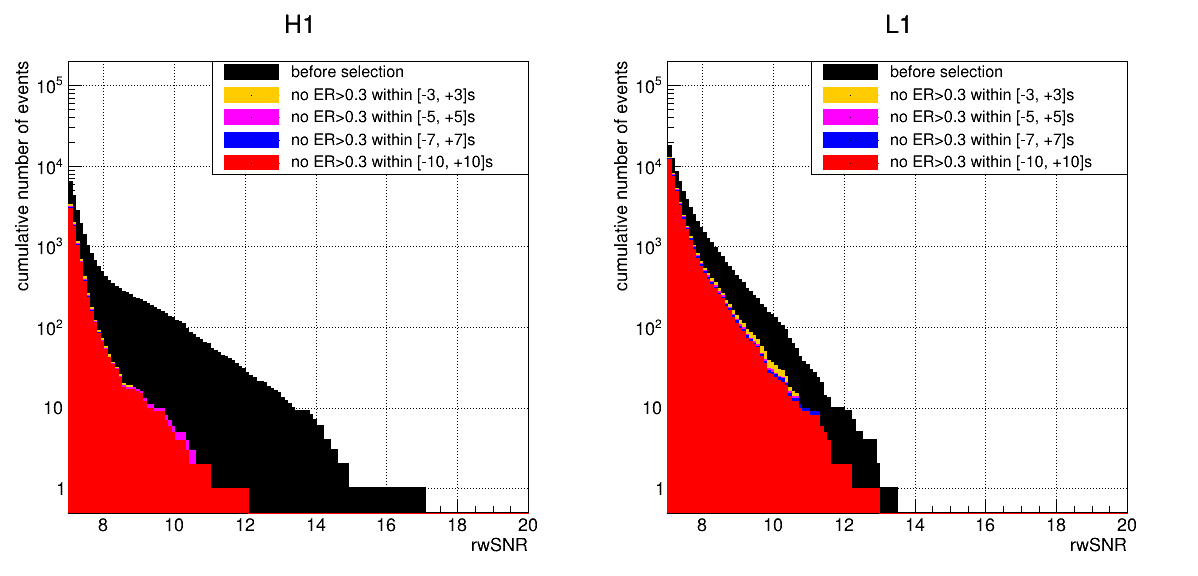
\includegraphics[width=\linewidth]{sectionO4/compareCutER_dark.png}
  \caption{Cumulative rwSNR distribution of long EM dark single detector triggers for the first 46.5 days of O4 (28.4 effective days in H1 and 38.7 effective days in L1) for several cuts on the excess rate. No selection on the gating is applied here. Triggers associated to significant public alerts were removed.}
  \label{fig:cutER_dark_O4}
\end{figure}
%
\begin{figure}
  \centering
  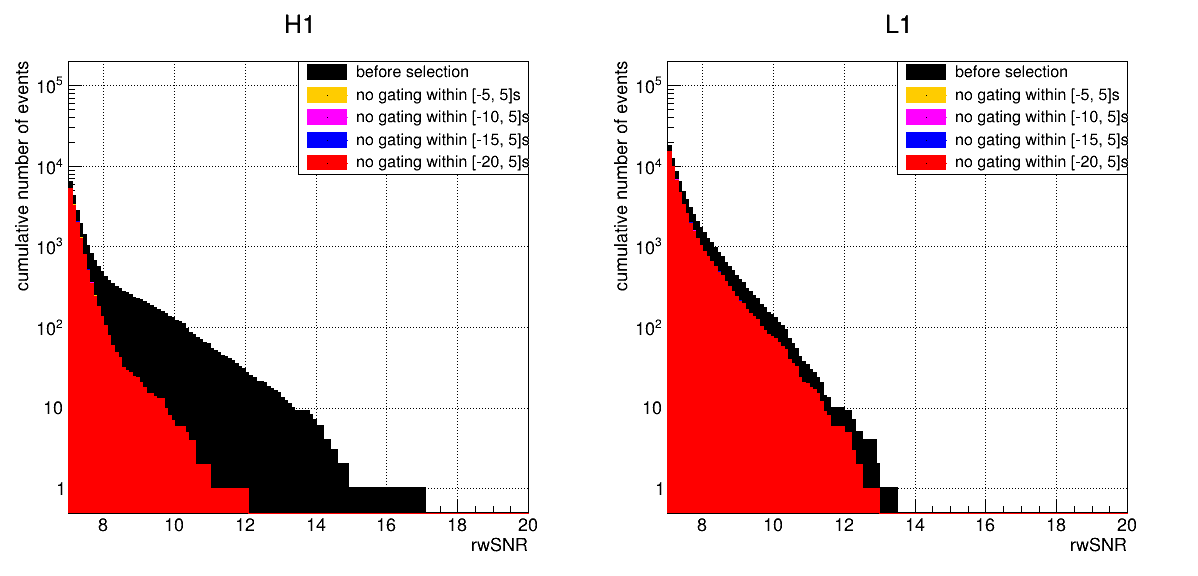
\includegraphics[width=\linewidth]{sectionO4/compareCutGating_dark.png}
  \caption{Cumulative rwSNR distribution of long EM dark single detector triggers for the first 46.5 days of O4 (28.4 effective days in H1 and 38.7 effective days in L1) for several cuts on the gating. No selection on the ER is applied here. Triggers associated to significant public alerts were removed.}
  \label{fig:cutGating_dark_O4}
\end{figure}



%%%%%%%%%%
\clearpage
\subsection{Background estimation for EM bright single detector triggers}

We now want to check that the method to compute background in order to estimate the FAR of candidates works satisfyingly.
We use for the estimation of the background $\sim 2.6$ days of effective observing time in H1 and $\sim 3.0$ in L1, from GPS = 1370250000 to GPS = 1370250000.
Figure \ref{fig:computed_bkg_O4} shows the background computed using trigger-random noise coincidences and trigger-trigger coincidences.
We see that on this period of time, the ``lower bound'' computed from random noise-random noise coincidences is actually higher than the observed single detector triggers.
It is not clear at this point whether this is simply a statistical effect due to the short duration used for the computation, or if it is a systematic effect.
This will require more investigation.
On the other side, the ``upper bound'', computed from trigger-trigger coincidences, behaves as expected from the work on O3 data.
The scaling factor in this is 6.3e-05 in H1 and 8.6e-05 in L1.
Both methods yield a background distribution of exponential shape with similar slope, we can extrapolate them.

Figure \ref{fig:cumulative_bkg_O4} shows the cumulative rwSNR distribution for the observed single detector triggers and the upper bound for the estimation of background.
The computed background is fitted with an exponential function $\text{FAR$_{8.6}$}\times\exp(\text{slope}(\text{rwSNR}-8.6))$.
The fit parameters are given in table \ref{tab:fitO4}.
We can also parametrize the rwSNR distribution of EM bright single detector triggers for the 46.5 days we showed previously.
The fitted function is not shown in figure \ref{fig:cumulative_bkg_O4} for readability but the parameters of the fit are given in table \ref{tab:fitO4}.
Although over-estimated, it allows to reach very low values for high rwSNR triggers.
%
\begin{table}[h]
  \centering
  \begin{tabular}{c|c|c|c|c|c}
    \multicolumn{6}{c}{Computed background (upper bound), fit from 8.5 to 9.5} \\ \hline
    Detector & FAR$_{8.6}$ (days$^{-1}$) & slope & IFAR$_8$ (days) & IFAR$_9$ (years) & IFAR$_{10}$ (centuries) \\ \hline
    H1 & 0.320 $\pm$ 0.004 & -7.32 $\pm$ 0.09 & 0.039 $\pm$ 0.002 & 0.160 $\pm$ 0.006 & 2.4 $\pm$ 0.3 \\
    L1 & 0.456 $\pm$ 0.004 & -6.56 $\pm$ 0.07 & 0.043 $\pm$ 0.002 & 0.083 $\pm$ 0.002 & 0.59 $\pm$ 0.06 \\
  \end{tabular}
\end{table}
  % 
\begin{table}[h]
  \centering
  \begin{tabular}{c|c|c|c|c|c}
    \multicolumn{6}{c}{Observed EM bright singles (46.5 days), fit from 7.5 to 8.5}\\ \hline
    Detector & FAR$_{8.6}$ (days$^{-1}$) & slope & IFAR$_8$ (days) & IFAR$_9$ (years) & IFAR$_{10}$ (centuries) \\ \hline
    H1 & 0.24 $\pm$ 0.02 & -7.01 $\pm$ 0.08 & 0.062 $\pm$ 0.002 & 0.19 $\pm$ 0.02 & 2.1 $\pm$ 0.4 \\
    L1 & 0.33 $\pm$ 0.02 & -6.29 $\pm$ 0.07 & 0.071 $\pm$ 0.002 & 0.10 $\pm$ 0.01 & 0.6 $\pm$ 0.1 \\
  \end{tabular}
  \caption{Results of the fit of the computed upper bound for the background and observed background over 46.5 days using $\text{FAR$_{8.6}$}\times\exp(\text{slope}(\text{rwSNR}-8.6))$.}
  \label{tab:fitO4}
\end{table}

\begin{figure}
  \centering
  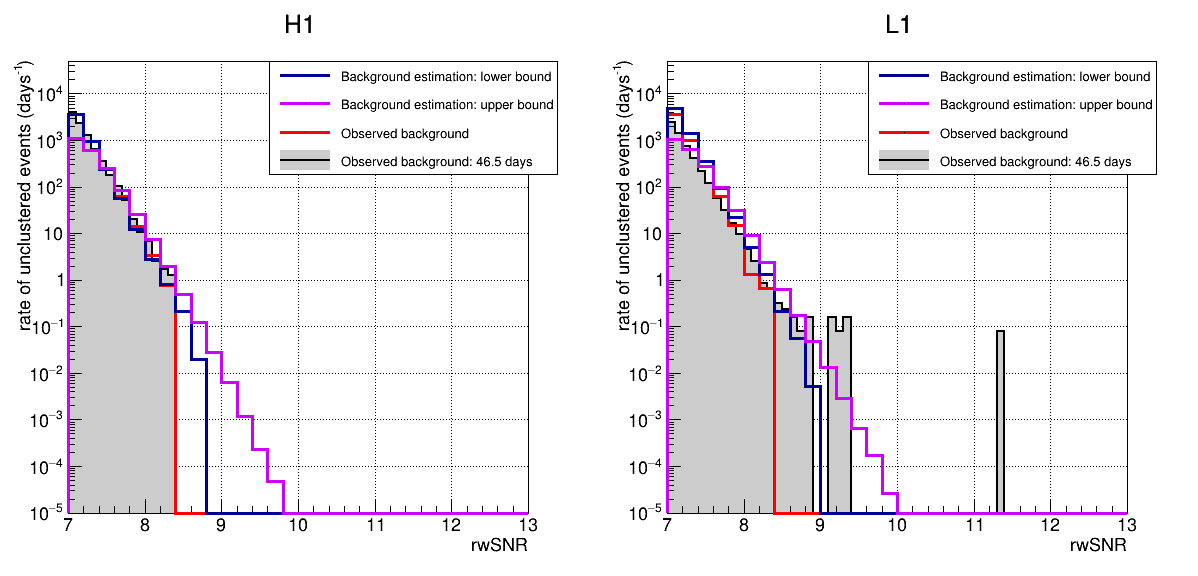
\includegraphics[width=\linewidth]{sectionO4/cPosterO4_HL.png}
  \caption{Comparison of the computed lower bound, upper bound and observed background for H1 (left) and L1 (right). Computation was done over $\sim 2.6$ and $\sim 3.0$ days for H1 and L1 respectively. All background are given for the EM bright population and the selection criteria are applied.}
  \label{fig:computed_bkg_O4}
\end{figure}
%
\begin{figure}
  \centering
  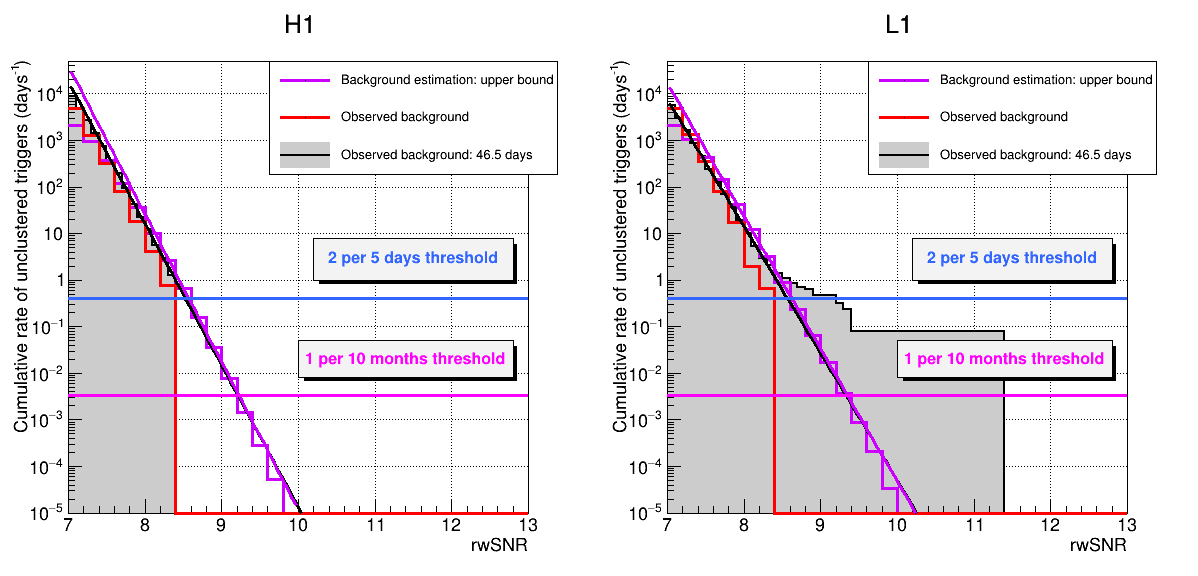
\includegraphics[width=\linewidth]{sectionO4/cPosterCumO4_HL.png}
  \caption{Comparison of the cumulative distributions of the observed background and computed upper bound for the background in H1 (left, for $\sim 2.6$ days of data) and L1 (right, for $\sim 3.0$ days of data) fitted with an exponential function. All background are given for the EM bright population and the selection criterai are applied.}
  \label{fig:cumulative_bkg_O4}
\end{figure}
